\documentclass[10pt]{article}

%==============================
% Document Metadata
%============================== 
\usepackage[pdftex,
    pdfauthor={Rukmal Weerawarana},
    pdftitle={Homework 3 Solutions - FE 621},
    pdfsubject={FE 621 - Computational Methods in Finance}
]{hyperref}


%==============================
% Package Imports
%==============================    
\usepackage[ruled]{algorithm2e} % typeset algorithms
\usepackage[authordate, maxcitenames=1]{biblatex-chicago} % chicago bibliography style
\usepackage{amsmath} % math environment stuff
\usepackage{amssymb} % additional math symbols
\usepackage[toc, page]{appendix} % Appendix referencing
\usepackage{booktabs} % Table lines
\usepackage{caption} % Caption formatting
\usepackage{comment} % enables the use of multi-line comments (\ifx \fi)
\usepackage[skip=5pt, labelfont=bf]{caption} % caption formatting
\usepackage{csvsimple} % CSV import to Table
\usepackage{enumitem} % Lists with alphabetical bullet points
\usepackage{fancyhdr} % Header
\usepackage{fancyvrb} % Verbatim text
\usepackage{float} % Controlling figure border
\usepackage[headings]{fullpage} % Set all margins to 1.5 cm
\usepackage{graphicx} % Figures
\usepackage{listings} % code embedding
\usepackage{longtable} % Multipage tables
\usepackage{multirow} % Multirow cells in tables
\usepackage{pmboxdraw} % Box characters for file tree
\usepackage{siunitx}  % SI units; float formatting
\usepackage[dvipsnames]{xcolor} % colors for code


%==============================
% Configuration
%==============================

% Figure outline configuration
% \floatstyle{boxed}
% \restylefloat{figure}

% Bibliography configuration

\addbibresource{../bibliography.bib}

% Remapping bibliography underscores (_) and tildes (~) because Mendeley has weird exporting
% Solution from: https://tex.stackexchange.com/questions/309980/parsing-underscores-in-urls-from-mendeley

\DeclareSourcemap{ % Used when .bib/Bibliography is compiled, not when document is
    \maps{
        \map{ % Replaces '{\_}', '{_}' or '\_' with just '_'
            \step[fieldsource=url,
                  match=\regexp{\{\\\_\}|\{\_\}|\\\_},
                  replace=\regexp{\_}]
        }
        \map{ % Replaces '{'$\sim$'}', '$\sim$' or '{~}' with just '~'
            \step[fieldsource=url,
                  match=\regexp{\{\$\\sim\$\}|\{\~\}|\$\\sim\$},
                  replace=\regexp{\~}]
        }
    }
}

% Code display configuration

\newcommand*\lstinputpath[1]{\lstset{inputpath=#1}} % Setting path
\lstset{
	language=Python,
	basicstyle=\footnotesize\ttfamily,
	commentstyle=\ttfamily\color{purple!40!black},
	identifierstyle=\color{blue},
	keywordstyle=\color{ForestGreen},
	numbers=left,
	numberstyle=\ttfamily\color{gray}\footnotesize,
	stepnumber=1,
	numbersep=5pt,
	backgroundcolor=\color{white},
	showspaces=false,
	showstringspaces=false,
	showtabs=false,
	frame=single,
	tabsize=2,
	captionpos=b,
	breaklines=true,
	breakatwhitespace=false,
	title=\lstname
}
\lstset{
	language=R,
	basicstyle=\footnotesize\ttfamily,
	commentstyle=\ttfamily\color{purple!40!black},
	identifierstyle=\color{blue},
	keywordstyle=\color{ForestGreen},
	numbers=left,
	numberstyle=\ttfamily\color{gray}\footnotesize,
	stepnumber=1,
	numbersep=5pt,
	backgroundcolor=\color{white},
	showspaces=false,
	showstringspaces=false,
	showtabs=false,
	frame=single,
	tabsize=2,
	captionpos=b,
	breaklines=true,
	breakatwhitespace=false,
	title=\lstname
}

% Header and Footer configuration

\pagestyle{fancy} % set page style
\fancyhead{} % override header
\fancyfoot{} % override footer
\renewcommand{\headrulewidth}{.4pt} % set header rule width 
\renewcommand{\footrulewidth}{.4pt} % set footer rule width 
\lhead{Homework Assignment 3} % set left header
\rhead{Rukmal Weerawarana} % set right header
\lfoot{\textit{FE 621}: Computational Methods in Finance} % set left footer
\rfoot{Page \thepage} % set right footer


%==============================
% Document Content
%==============================

\begin{document}

\thispagestyle{plain}

\pagenumbering{roman}  % Changing numbering to Roman numerals for first pages

%==============================
% Document Title
%==============================

\noindent
\large\textbf{Homework Assignment 3} \hfill \textbf{Rukmal Weerawarana} \\
\normalsize \textit{FE 621}: Computational Methods in Finance \hfill \textit{rweerawa@stevens.edu} $\mid$ 104-307-27 \\
\textit{Instructor}: Ionut Florescu \hfill Department of Financial Engineering \\
4/21/2019 \hfill Stevens Institute of Technology

\noindent\rule{\linewidth}{.1em}
\pagenumbering{arabic}  % Changing numbering to arabic numerals for main content

%==============================
% Q1 - Quadratic Volatility Model
%==============================

\section{Quadratic Volatility Model}

\subsection{Part (a)}

Analyzing Figure~\ref{fig:quad_vol}, it is clear that the transition density increases commensurately with converging values of $x$ and $x_0$.

Additionally, the transition density appears to increase significantly as the time to maturity, $t$ decreases. This is particularly evident when comparing the maximum values of Figure~\ref{fig:quad_vol} Panel (a) to Figure~\ref{fig:quad_vol} Panel (d), whose maximum volatility transition density appears to be barely half of that of Panel (a) at its peak.

\subsection{Part (b)}

\begin{table}[!h]
    \centering
	\csvautotabular{bin/q1_finite_diff_approx_verification.csv}
\end{table}

Verifying that the finite difference approximation of the transition probability density satisfies the initial Partial Differential Equation. The absolute value of the difference between the Finite Difference approximation and the PDE value is displayed above.

\subsection{Part (c)}

\begin{table}[!h]
    \centering
    \csvautotabular{bin/q1_call_option_prices.csv}
    \caption{European Call Option priced with the Quadratic Volatility and Black Scholes models.}
    \label{table:q1:opt_prices}
\end{table}



\section{Fast Fourier Transform}

\begin{table}[!h]
    \centering
    \csvautotabular[respect all]{bin/q2_price_comparison.csv}
    \caption{European Call Option priced with the Fast Fourier Transform and Black Scholes models.}
    \label{table:q2:fft_prices}
\end{table}



\pagebreak

\begin{figure}[]
	\centering
	\begin{tabular}{|c|c|}
		\hline
		{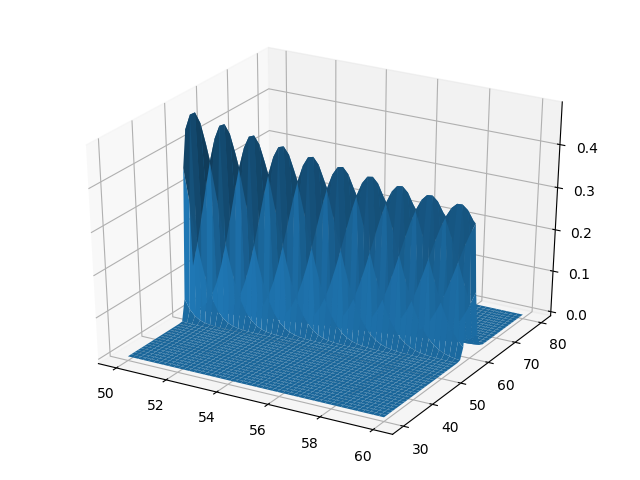
\includegraphics[width=.475\linewidth]{bin/q1_quadvol_t_10}} & 
		{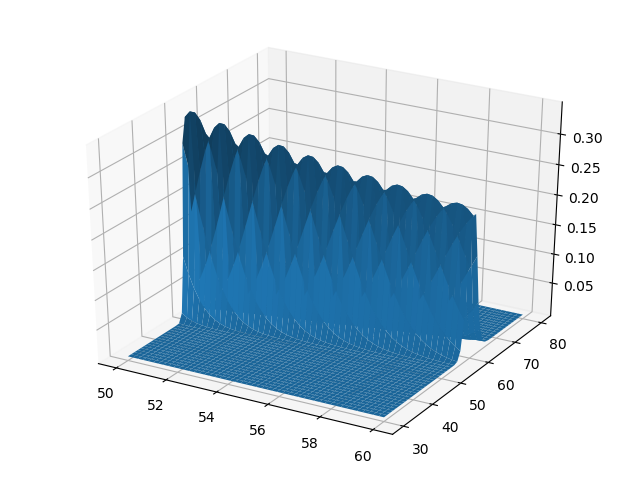
\includegraphics[width=.475\linewidth]{bin/q1_quadvol_t_20}}\\
		{(a) $t = 10$} & {(b) $t = 20$} \\
		\hline
		{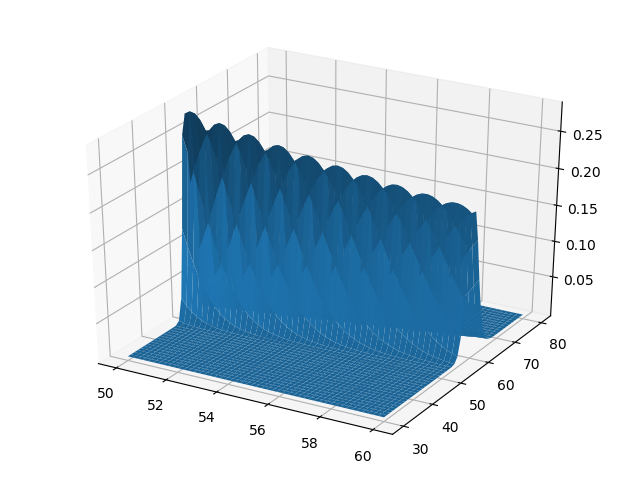
\includegraphics[width=.475\linewidth]{bin/q1_quadvol_t_30}} &
		{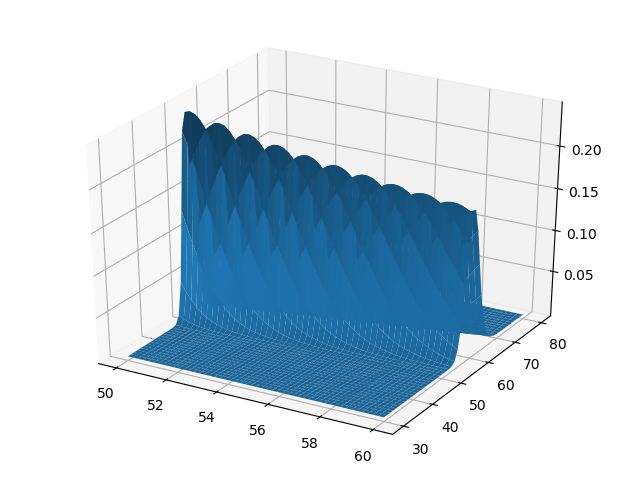
\includegraphics[width=.475\linewidth]{bin/q1_quadvol_t_40}} \\
		{(c) $t = 30$} & {(d) $t = 40$} \\
		\hline
	\end{tabular}
	\captionof{figure}{Surface plots of Quadratic Volatility Models with varying times, $t$.}
	\label{fig:quad_vol}
\end{figure}


%==============================
% APPENDIX
%==============================
\clearpage

% Resetting input path
\lstinputpath{}

\newpage
\section{Solution Source Code} \label{appendix:source}
    \subsection{Question 1 Solution} \label{appendix:source:q1}
		\subsubsection{Quadratic Volatility Plots}
			\lstinputlisting{question_solutions/q1_qvol_plots.py}

		\subsection{Call Option Pricing}
			\lstinputlisting{question_solutions/q1_call_option.py}

    \subsection{Question 2 Solution} \label{appendix:source:q2}
		\lstinputlisting{question_solutions/q2_fft.py}

%==============================
% REFERENCES
%==============================
\newpage

\nocite{Shreve2004}
\nocite{Stefanica2011}
\nocite{Weerawarana2016}
\nocite{Florescu2019}
\nocite{Carr}

\printbibliography

%==============================
% Document End
%==============================

\end{document}
